%!TeX root=../tese.tex
%("dica" para o editor de texto: este arquivo é parte de um documento maior)
% para saber mais: https://tex.stackexchange.com/q/78101

%% ------------------------------------------------------------------------- %%

\unnumberedchapter{Introdução}
{\color{red} Em andamento}


\label{cap:introducao}
\enlargethispage{.5\baselineskip}
A hemofilia é uma doença hereditária rara, caracterizada por uma deficiência nos fatores de coagulação sanguínea. Existem dois principais tipos de hemofilia: a A, causada pela deficiência do fator VIII de coagulação, e a hemofilia B, causada pela deficiência do fator IX. 
Os pacientes com hemofilia enfrentam um risco maior de sofrer com hemorragias graves, tanto internas quanto externas, 
podendo levar a complicações debilitantes e até mesmo à morte \cite{Mannucci}.

Embora tenham sido obtidos avanços notáveis no tratamento da doença nas últimas décadas, muitos desafios ainda persistem \cite{Gouw}. 
O tratamento tradicional da hemofilia envolve a infusão de fatores de coagulação recombinantes ou derivados do plasma sanguíneo \cite{Gouw}. Apesar de sua eficácia na prevenção de hemorragias, esse tratamento possui limitações, tais como a necessidade de infusões frequentes, a possibilidade de desenvolvimento de inibidores anticoagulantes e, principalmente, os altos custos envolvidos \cite{Mancuso}. 
{\color{red} Pegar algum artigo que fale sobre a instabilidade do fator IX, que faz com que o tratamento seja caro e sobre a resposta imune.}
O projeto de sequências proteicas surge como uma abordagem que tem potencial de reduzir substancialmente os custos associados ao tratamento da doença, ao criar proteínas sob medida com eficácia comparável.

\begin{figure}[H]
  \centering
  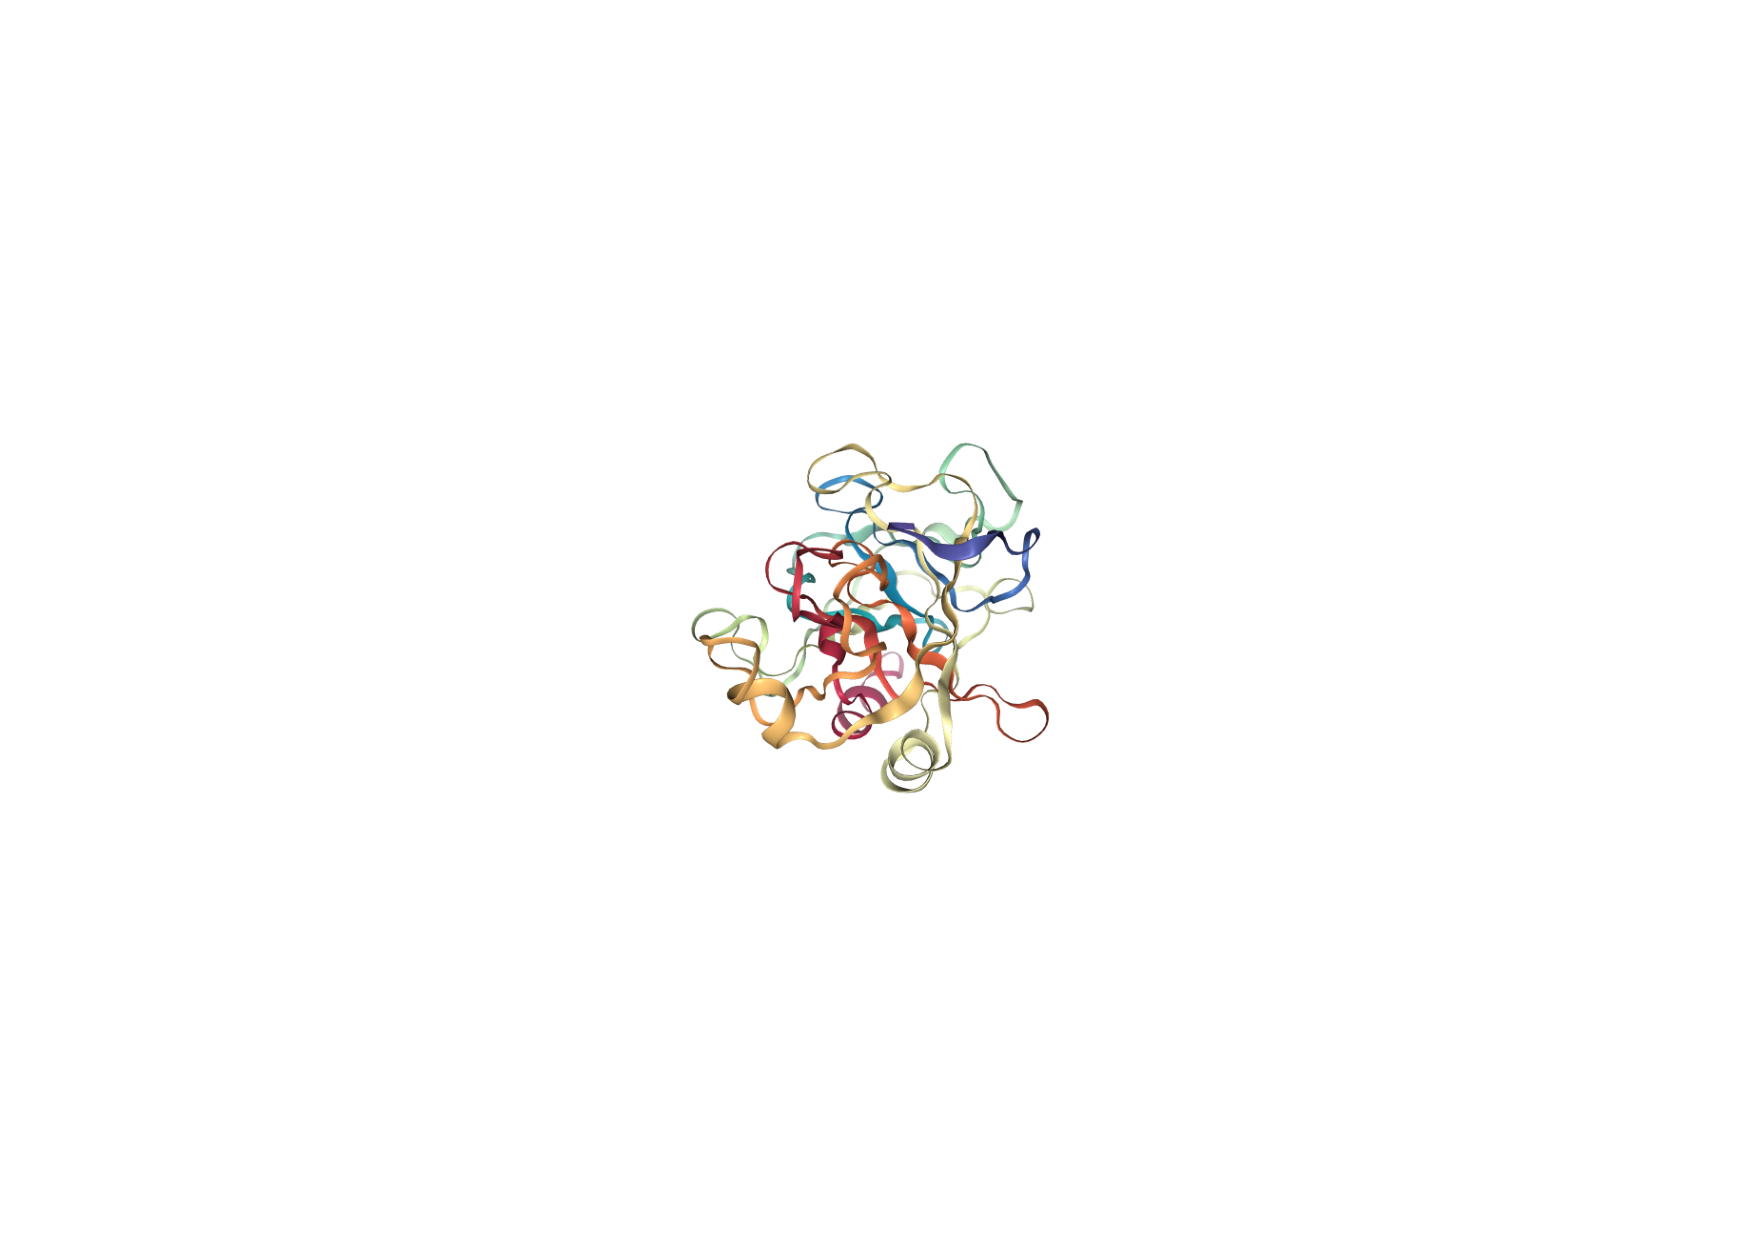
\includegraphics[width=.8\textwidth]{figuras/target_structure.pdf}
  \caption{Estrutura Alvo: Fator IX - Hemofilia tipo B}
\end{figure}


\section{Projeto de sequências}
%%%%%%%%%%%%%%%%%%%%%%%%%%%%%%%%%%%%%%%%%%%%%%%%%%%%%%%%%%%%%%%%%%%%%%%%%%%%%%%%%%%%%%%%%%%%%%%%%%%%%%%%%%%%%%%%%%%%%%%%%%%%%%%%%%%%%%%%%%%%%%%%%%%%%%%%%%%%%%%%
%Falar do The coming of age of de novo protein design 
%Falar do Computational protein design
%%%%%%%%%%%%%%%%%%%%%%%%%%%%%%%%%%%%%%%%%%%%%%%%%%%%%%%%%%%%%%%%%%%%%%%%%%%%%%%%%%%%%%%%%%%%%%%%%%%%%%%%%%%%%%%%%%%%%%%%%%%%%%%%%%%%%%%%%%%%%%%%%%%%%%%%%%%%%%%%

O projeto de sequências se refere ao processo de criar ou otimizar uma sequência de aminoácidos de modo a produzir uma proteína cuja estrutura tridimensional possua características desejadas. Esta é uma tarefa desafiadora que, a depender do tamanho da sequência, é inviável de se resolver através de uma busca por força bruta, devido as inúmeras permutações possíveis que se pode obter com os 20 aminoácidos conhecidos na natureza \cite{Overview}.  

\begin{figure}[H]
  \centering
  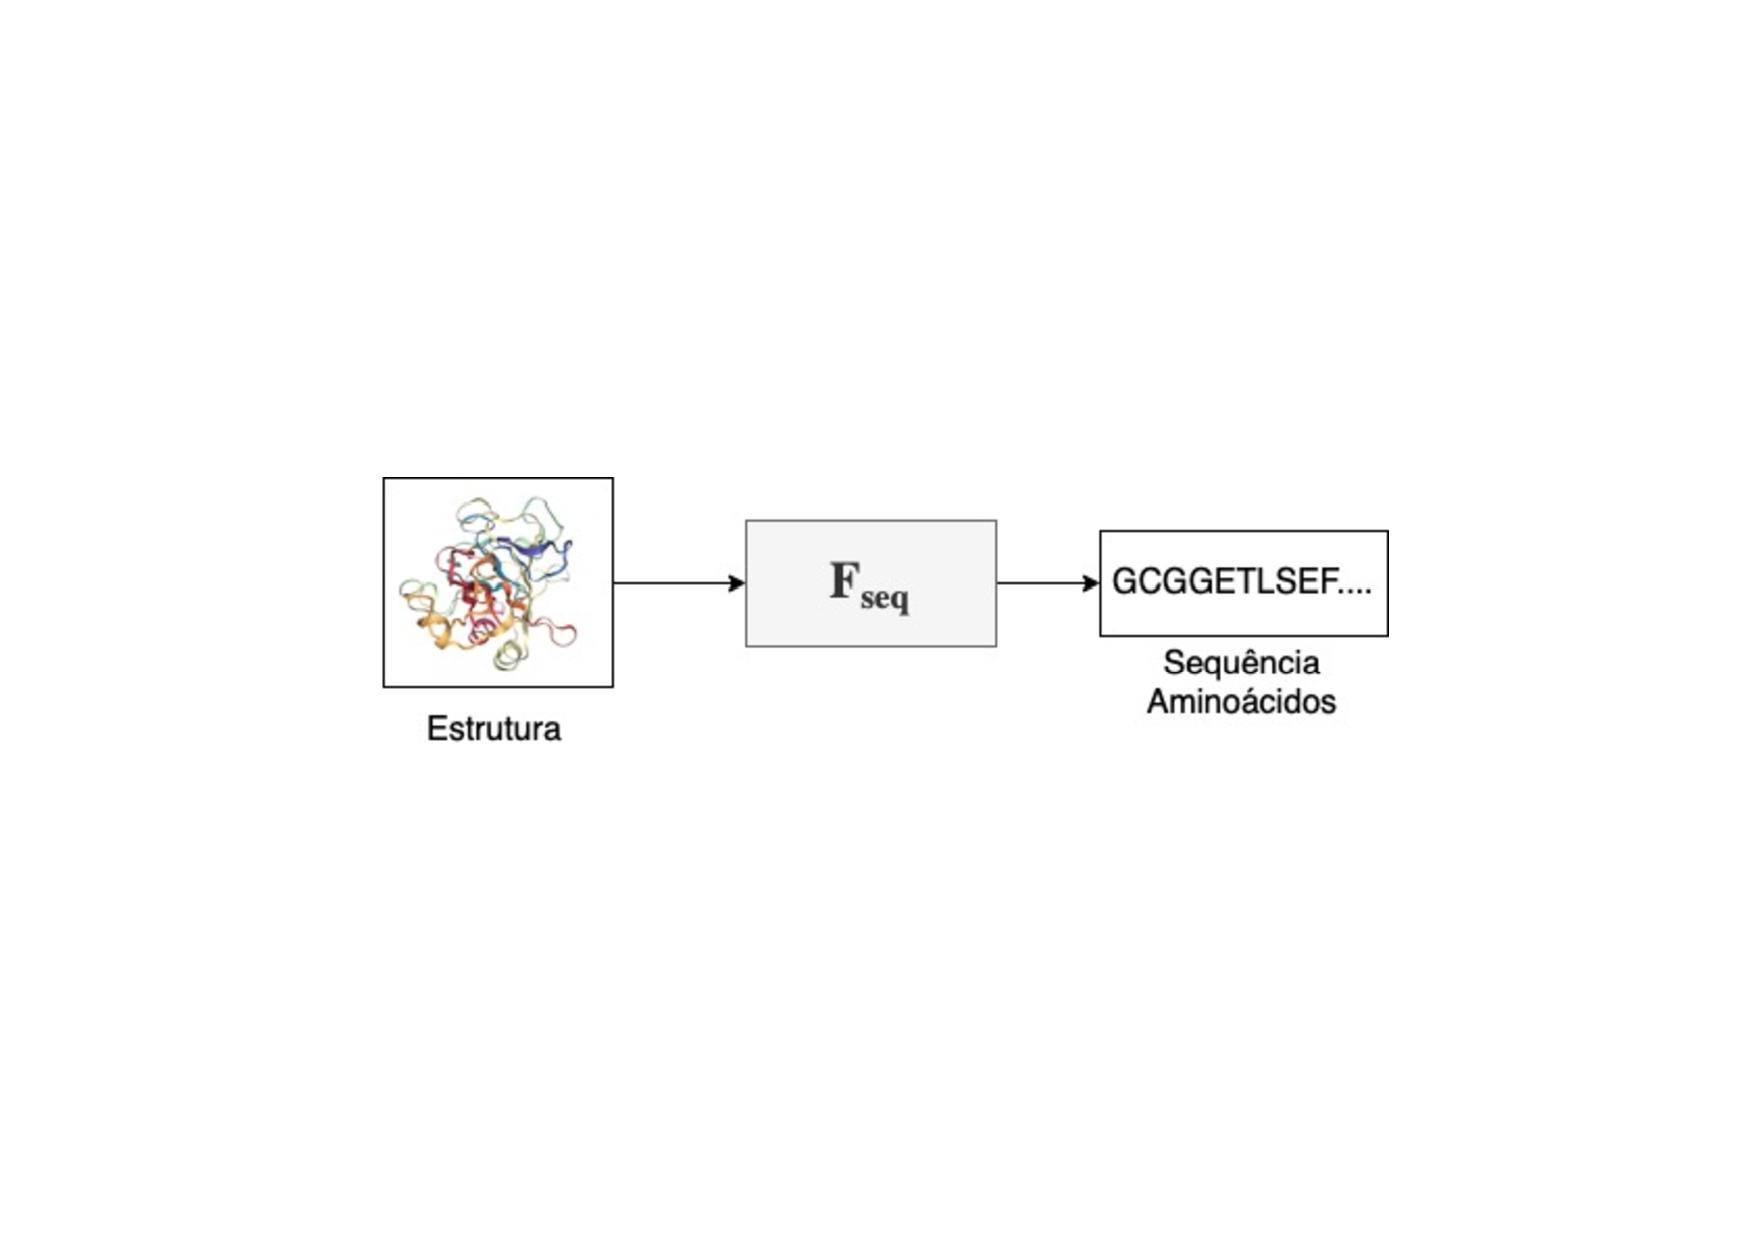
\includegraphics[width=.8\textwidth]{figuras/metodologia-SeqDes.pdf}
  \caption{Projeto de Sequências}
  O projeto de sequências se resume a desenvolver uma função $F_{seq}$ que mapeia uma estrutura protéica tridimensional em uma sequência de aminoácidos. 
\end{figure}


\subsection{Baseado em busca}
O projeto de sequências baseado em busca, em geral, define a função $F_{seq}$ através do seguinte pipeline:

\begin{enumerate}
  \item Dada uma estrutura proteíca, é definida uma sequência de aminoácidos inicial, baseada em uma  heurística $H$.
  \item A sequência serve de entrada para a função objetivo $F_{obj}$ que calcula a métrica a ser otimizada pelo pipeline.
  \item Se a sequência atual é melhor do que sequência final, em termos da métrica calculada pela $F_{obj}$, então o Agente $A$ define a sequência atual como a nova sequência final. Além disso, $A$ também atualiza a sequência atual a partir de mutações.
  \item O processo se repete a partir do item 2 até que seja atingido um critério de parada. Geralmente é baseado no número de iterações e/ou na métrica objetivo. 
\end{enumerate}

\begin{figure}[H]
  \centering
  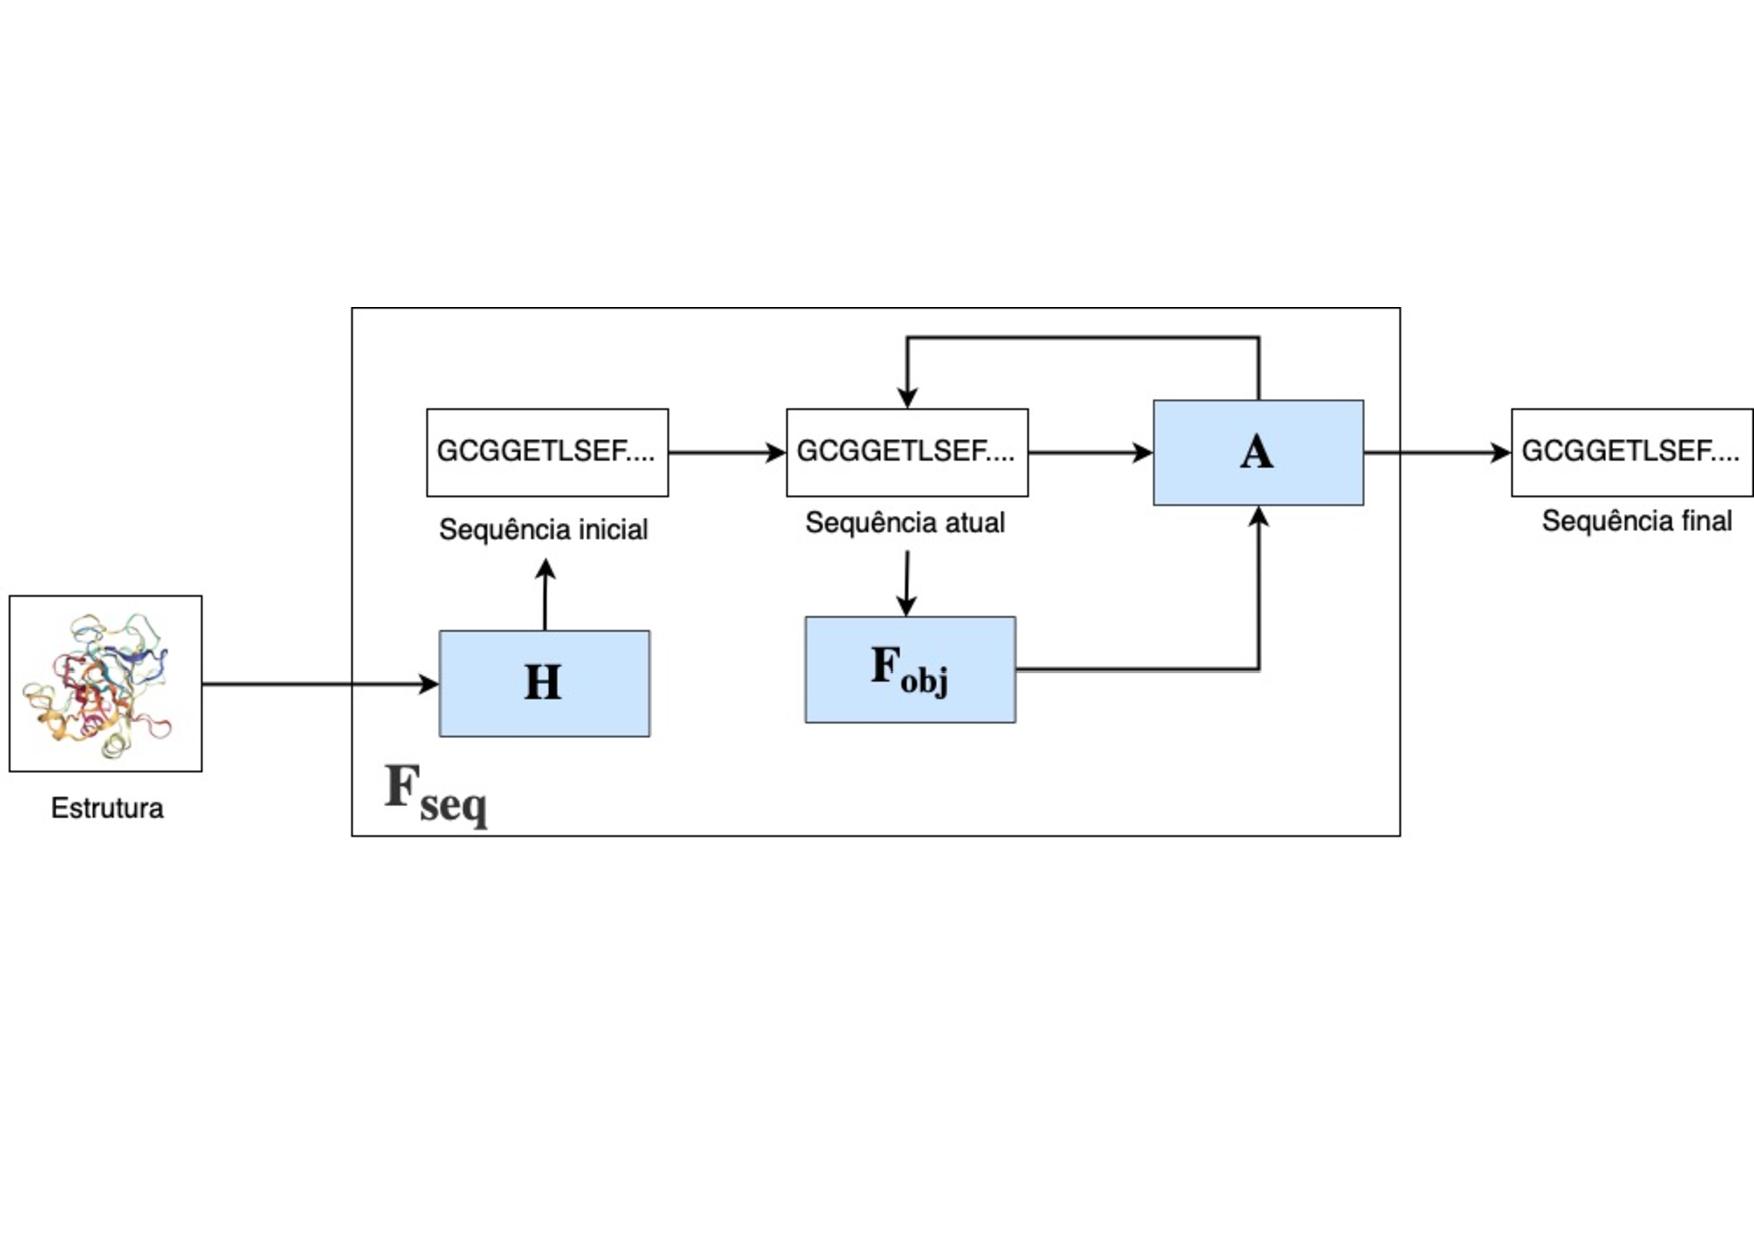
\includegraphics[width=.8\textwidth]{figuras/metodologia-SearchBased.pdf}
  \caption{Projeto de Sequências baseado em busca} 
  \label{fig:seqdes_search_based}
\end{figure}

%Falar que a função objetivo pode ser energia, como o Rosetta, ou tambem pode ser em similariedade 
%%%%%%%%%%%%%%%%%%%%%%%%%%%%%%%%%%%%%%%%%%%%%%%%%%%%%%
%%%%%%%%%%%%%%%%%%%%%%%%TO DO %%%%%%%%%%%%%%%%%%%%%%%%
%%%%%%%%%%Fazer um fichamento sobre o Rosetta e garantir que oq esta escrito esta correto e suficiente%%%%%%%%%
%%%%%%%%%%%%%%%%%%%%%%%%%%%%%%%%%%%%%%%%%%%%%%%%%%%%%%
%Rosetta

O \textit{Rosetta} \cite{Rosetta} se baseia em um pipeline como este, onde a heurística $H$ define como partida uma sequência de uma proteína homóloga ou estruturalmente semelhante a estrutura alvo.  
Sua função objetivo $F_{obj}$ mede a energia livre da proteína, considerando diversos fatores como interações de \textit{Van der Waals}, interações eletrostáticas, ligações de hidrogênio, solubilidade, entre outros. 
O \textit{Rosetta} busca minimizar a energia livre calculada pela $F_{obj}$. Portanto, seu Agente $A$ 
decide que a sequência final passa a ser a atual se houver um decréscimo na energia livre. Além disso, atribui modificações na sequência atual de forma aleatória, utilizando o Método de Monte Carlo (MMC).

%Confirmar se vamos manter isso aqui

{\color{red} Existem abordagens cujo o objetivo da busca se concentra em maximizar a similaridade entre as proteínas, como adotado por xx. Com o objetivo de criar novas proteínas nunca antes vistas na natureza, \cite{DeNovo} parte de uma sequência aleatória de aminoácidos, i.e, não possui uma heurística inicial. A função $M$, assim como o \textit{Rosetta}, consiste de um MCC. Já a função objetivo $F_{obj}$ calcula a divergência de \textit{Kullback-Leibler} entre ...}



\subsection{Baseado em aprendizado profundo}

O projeto de sequências baseado em aprendizado profundo define a função $F_{seq}$ a partir de redes neurais artificiais. 
O \cite{ProteinMPNN} por exemplo, determina a $F_{seq}$ como uma rede neural profunda, denominada \textit{ProteinMPNN}, 
que mapeia de forma direta a estrutura alvo à sequência de aminoácidos. 
A rede é construída através de uma \textit{Message Passing Neural Network} (MPNN) composta por uma arquitetura \textit{encoder-decoder} 
que se baseia nas características da estrutura - distância e orientação dos átomos no espaço - para fazer predições \cite{ProteinMPNN}. 

\begin{figure}[H]
  \centering
  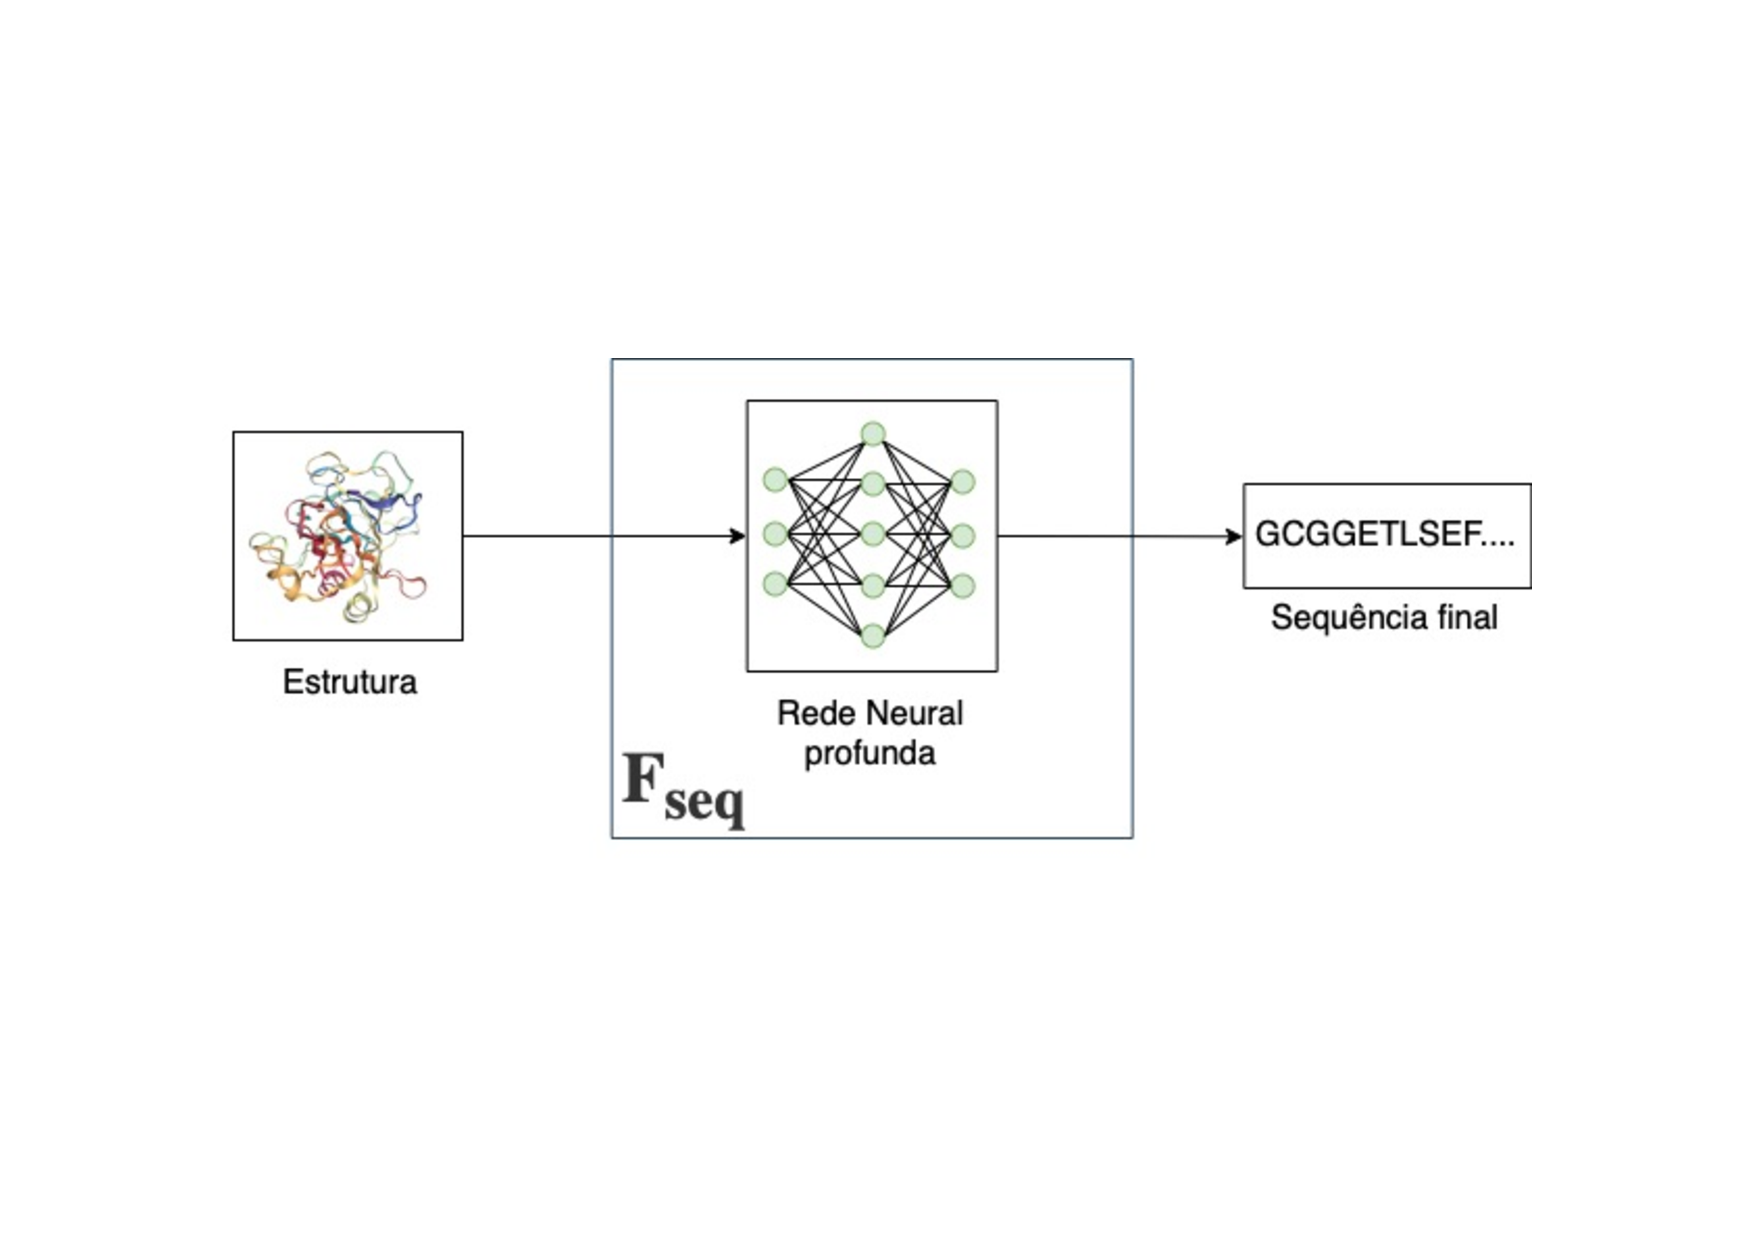
\includegraphics[width=.8\textwidth]{figuras/metodologia-DeepLearningBased.pdf}
  \caption{Projeto de Sequências baseado em aprendizado profundo} 
\end{figure}

{\color{red} Falar sobre o RL in latent space e mencionar alg. genetico}

\section{Proposta} 
\label{section:Proposta}
%Problema: tratamento com Fator IX é caro por exigir inumeras infusoes pq o Fator IX é instavel. Alem disso, pode gerar resposta imune nos pacientes. 
%A pergunta cientifica é: É possível encontrar uma proteina melhor (mais estavel, mais barata de se produzir, menos resposta imune e capaz de exercer as mesmas funções da proteina original) que a proteina original utilizando um pipeline de busca, com RL, otimizando TMScore?
%A nossa hipótese é que, se houver uma proteína melhor que desempenha a mesma função, ela deve ter uma estrutura tridimensional similar. Logo, a busca será feita no espaço de proteínas similares. Logo, criamos um pipeline para gerar um conjunto de proteínas candidatas. 
Além de possívelmente provocar uma resposta imune no paciente, o tratamento da hemofilia tipo B, baseado na infusão do Fator IX, é custoso devido ao pouco tempo de vida do Fator IX na corrente sanguínea, demandando infusões frequentes. 
Neste sentido, o presente trabalho se propõe a responder a seguinte pergunta científica: É possível, através de projeto de sequências, projetar uma proteína que desempenhe a mesma função do Fator IX mas com um perfil imunológico melhor e que demande menos infusões no tratamento da hemofilia tipo B?

Para responder a esta questão, formulamos a hipótese de que, se existir uma proteína alternativa superior ao Fator IX, ela deverá ser estruturalmente similar. Com base nisso, pretendemos selecionar, dentre um conjunto de proteínas estruturalmente semelhantes ao Fator IX, aquelas que satisfaçam os critérios estabelecidos, caso existam.

De modo a obter esse conjunto de proteínas, será desenvolvido um pipeline que combina a arquitetura do projeto de sequências baseado em busca e técnicas de aprendizado profundo.
O processo será dividido em três módulos: Condições Iniciais, Treinamento e Geração de Sequências. 

O módulo de Condições iniciais consiste na obtenção da sequência inicial de aminoácidos através da heurística $H$, bem como o cálculo do erro inicial associado a esta sequência, usando a função objetivo $F_{obj}$. 
Vamos utilizar o \textit{ProteinMPNN} como heurística $H$ e a métrica de similaridade estrutural \textit{Template Matching Score} (\textit{TMScore}) como função objetivo.

Diferente do uso de agentes que realizam mutações aleatórias, como no \textit{Rosetta}, no módulo de Treinamento, treinaremos uma rede neural profunda para atuar como o Agente $A$,
capaz de realizar mutações que otimizem a similaridade com a estrutura alvo, isto é, o Fator IX.

Após o treinamento, no módulo de Geração de Sequências, 
espera-se que o Agente seja capaz de gerar várias proteínas estruturalmente semelhantes à estrutura alvo por meio de mutações direcionadas. 
A partir das sequências geradas, avaliaremos a existência de candidatas viáveis para substituir o Fator IX no tratamento da hemofilia tipo B.



\begin{figure}[H]
  \centering
  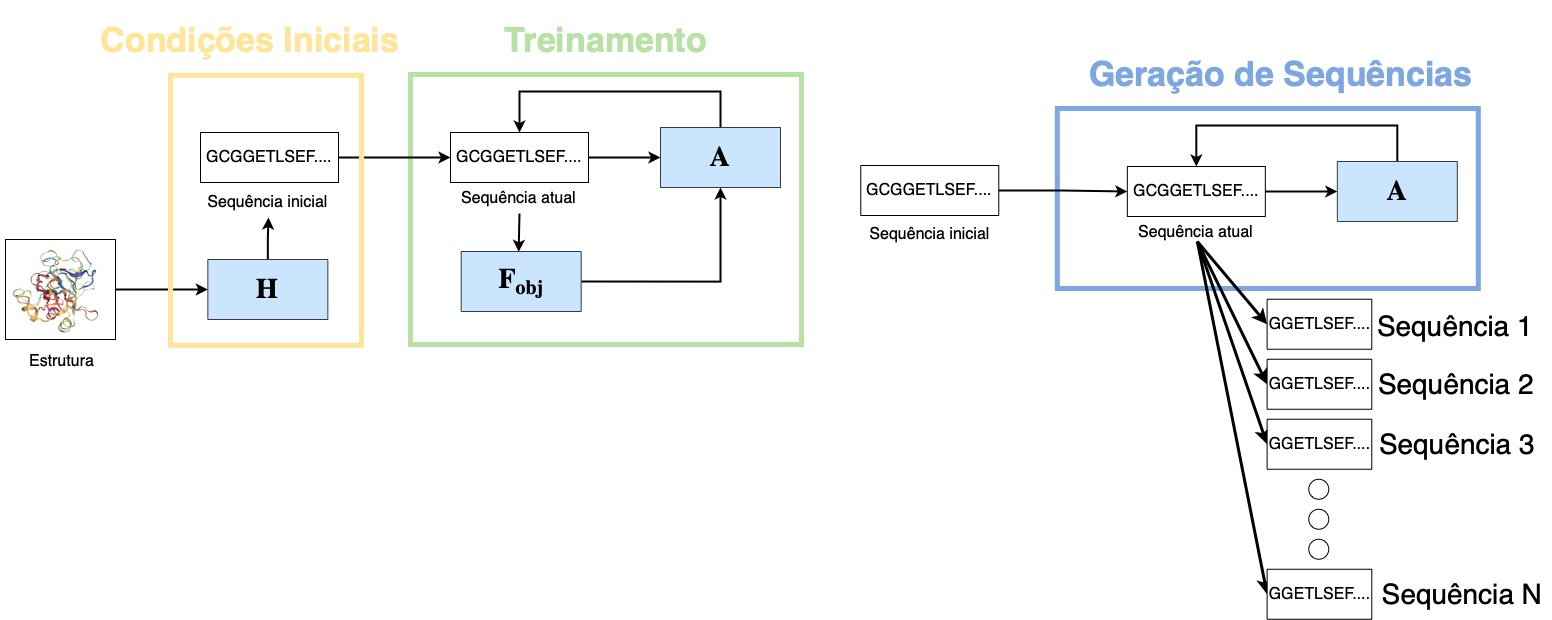
\includegraphics[width=.8\textwidth]{figuras/metodologia-pipeline_proposta.jpg}
  \begin{itemize}
  \item o \textit{ProteinMPNN} será utilizado como heurística $H$. 
  \item Na função objetivo $F_{obj}$ será calculada uma métrica de similaridade entre a estrutura da proteína atual 
  e a estrutura alvo que pretendemos maximizar: \textit{Template Matching Score} - \textit{TMScore}.
  \item O Agente $A$ será uma rede neural profunda, nomeada de  \textit{GenSeq},
  treinada para receber uma sequência de aminoácidos e prever a mutação que maximiza a similaridade com a estrutura alvo, i.e, otimiza $F_{obj}$. 
  O treinamento do $A$ será feito com aprendizado por reforço profundo, utilizando a ténica \textit{Proximal Policy Optimization} - PPO
  \item Depois de treinado, $A$ será utilizado como gerador de proteínas estruturalmente semelhantes ao Fator IX. 
\end{itemize}
  \caption{Projeto de Sequências proposto} 
  \label{fig:proposta}
\end{figure}

\section{Objetivos} 

Definimos os seguintes objetivos:

\begin{enumerate}
  \item Obter um conjunto de sequências de aminoácidos que mimetizem a estrutura do fator de coagulação IX baseado na métrica TM-Score.
  \item Avaliar, dentro do conjunto de proteínas obtidas em 1, quais possuem potencial de substituir o Fator IX de modo tornar o tratamento de Hemofilia tipo B mais acessível.
  \item Desenvolver um \textit{pipeline} genérico que produza sequências que mimetizem uma estrutura qualquer.
\end{enumerate}






 
